%%%%%%%%%%%%%%%%%%%%%%%%%%%%%%%%%%%%%%%%%%%%%%%%%%%%
%                 CONCLUSIÓN INTUITIVA 
%      para poder finiquitar la memoria a tiempo
%%%%%%%%%%%%%%%%%%%%%%%%%%%%%%%%%%%%%%%%%%%%%%%%%%%%

\section{Utilidad del algoritmo de inicialización de pesos en problemas de teoría de la aproximación clásicos}

El algoritmo que acabamos de implementar no solo 
tiene su utilidad en el uso de inicialización de pesos 
de redes neuronales, sino que resuelve problemas 
de teoría de aproximación clásicos. 

Para mostrar esto habrá que remontarse a los ejemplos
del comienzo de este trabajo.  
En la sección \ref{ch03:conclusiones-teoria-aproximacion}
se mostraba que había algunas funciones cuyo error
de aproximación  tendía a infinito.
Gracias al teorema \ref{teo:MFNAUA} sabemos que 
las redes neuronales convergen llevando el error 
a cero. 

Véase cómo se aproxima ahora el ejemplo patológico
que se mostraba en la figura \ref{fig:aproximacion-lagrage}: 

\begin{figure}[H]
    \centering
    \begin{subfigure}[b]{0.475\textwidth}
        \centering
        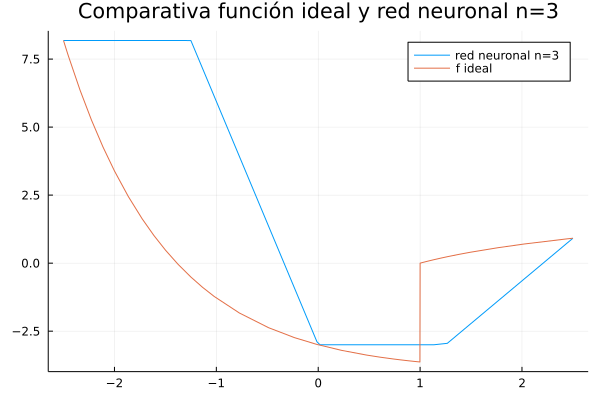
\includegraphics[width=\textwidth]{7-algoritmo-inicializar-pesos/f_ideal_y_rn_con_3_neuronas.png}
        \caption[Network2]%
        {{\small Red neuronal inicializada a partir de 3 datos}}    
    \end{subfigure}
    \hfill
    \begin{subfigure}[b]{0.475\textwidth}  
        \centering 
        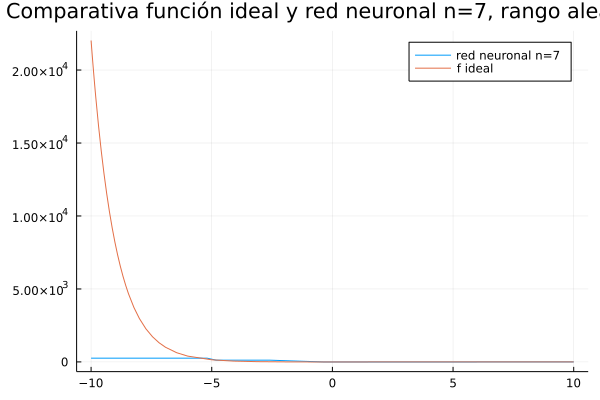
\includegraphics[width=\textwidth]{7-algoritmo-inicializar-pesos/f_ideal_y_rn_con_7_neuronas.png}
        \caption[]%
        {{\small Red neuronal inicializada a partir de 7 datos}}    
    \end{subfigure}
    \vskip\baselineskip
    \begin{subfigure}[b]{0.475\textwidth}   
        \centering 
        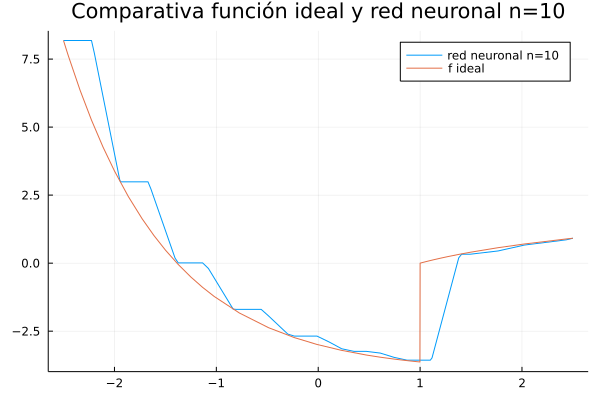
\includegraphics[width=\textwidth]{7-algoritmo-inicializar-pesos/f_ideal_y_rn_con_10_neuronas.png}
        \caption[]%
        {{\small Red neuronal inicializada a partir de 10 datos}}    
    \end{subfigure}
    \hfill
    \begin{subfigure}[b]{0.475\textwidth}   
        \centering 
        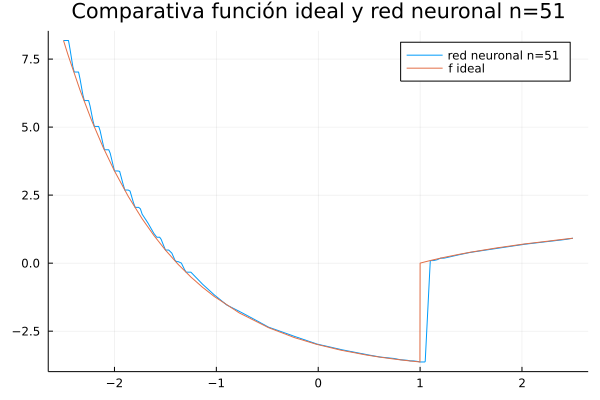
\includegraphics[width=\textwidth]{7-algoritmo-inicializar-pesos/f_ideal_y_rn_con_51_neuronas.png}
        \caption[]%
        {{\small Red neuronal inicializada a partir de 51 neuronas}}    
    \end{subfigure}
    \caption{Ejemplo de aproximación de la función $f(x)$ con redes neuronales.} 
    \label{fig:aproximacion-red-neuronal}
\end{figure}
\begin{figure}[H]
    \centering
     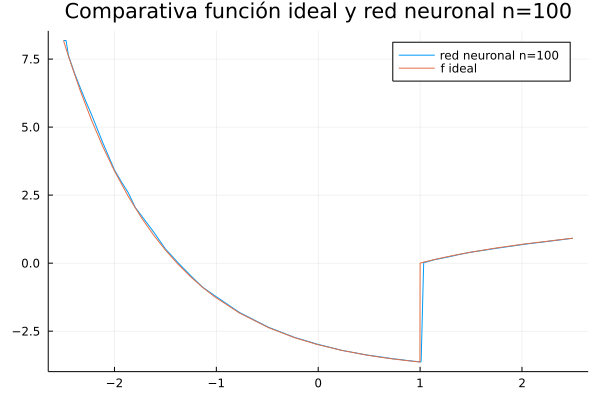
\includegraphics[width=.5\textwidth]{7-algoritmo-inicializar-pesos/f_ideal_y_rn_con_100_neuronas.png}
     \caption{Ejemplo de aproximación de la función $f(x)$ con red neuronal de 100 neuronas.}
     \label{fig:aproximacion-red-neuronal-2}
    \end{figure}
